\documentclass{beamer}
\mode<presentation>
\usepackage{amsmath}
\usepackage{amssymb}
%\usepackage{advdate}
\usepackage{adjustbox}
\usepackage{subcaption}
\usepackage{enumitem}
\usepackage{multicol}
\usepackage{mathtools}
\usepackage{listings}
\usepackage{url}
% \usepackage{minted}
% \usepackage{gvv}

\usepackage{tcolorbox}
\tcbuselibrary{minted,breakable,xparse,skins}



\definecolor{bg}{gray}{0.95}
\DeclareTCBListing{mintedbox}{O{}m!O{}}{%
  breakable=true,
  listing engine=minted,
  listing only,
  minted language=#2,
  minted style=default,
  minted options={%
    linenos,
    gobble=0,
    breaklines=true,
    breakafter=,,
    fontsize=\scriptsize,
    numbersep=8pt,
    #1},
  boxsep=0pt,
  left skip=0pt,
  right skip=0pt,
  left=25pt,
  right=0pt,
  top=3pt,
  bottom=3pt,
  arc=5pt,
  leftrule=0pt,
  rightrule=0pt,
  bottomrule=2pt,
  toprule=2pt,
  colback=bg,
  colframe=orange!70,
  enhanced,
  overlay={%
    \begin{tcbclipinterior}
    \fill[orange!20!white] (frame.south west) rectangle ([xshift=20pt]frame.north west);
    \end{tcbclipinterior}},
  #3,
}


\def\UrlBreaks{\do\/\do-}
\usetheme{Madrid}
\usecolortheme{lily}
\setbeamertemplate{footline}
{
  \leavevmode%
  \hbox{%
  \begin{beamercolorbox}[wd=\paperwidth,ht=2.25ex,dp=1ex,right]{author in head/foot}%
    \insertframenumber{} / \inserttotalframenumber\hspace*{2ex} 
  \end{beamercolorbox}}%
  \vskip0pt%
}
\setbeamertemplate{navigation symbols}{}

\providecommand{\nCr}[2]{\,^{#1}C_{#2}} % nCr 
\providecommand{\nPr}[2]{\,^{#1}P_{#2}} % nPr
\providecommand{\mbf}{\mathbf}
\providecommand{\pr}[1]{\ensuremath{\Pr\left(#1\right)}}
\providecommand{\qfunc}[1]{\ensuremath{Q\left(#1\right)}}
\providecommand{\sbrak}[1]{\ensuremath{{}\left[#1\right]}}
\providecommand{\lsbrak}[1]{\ensuremath{{}\left[#1\right.}}
\providecommand{\rsbrak}[1]{\ensuremath{{}\left.#1\right]}}
\providecommand{\brak}[1]{\ensuremath{\left(#1\right)}}
\providecommand{\lbrak}[1]{\ensuremath{\left(#1\right.}}
\providecommand{\rbrak}[1]{\ensuremath{\left.#1\right)}}
\providecommand{\cbrak}[1]{\ensuremath{\left\{#1\right\}}}
\providecommand{\lcbrak}[1]{\ensuremath{\left\{#1\right.}}
\providecommand{\rcbrak}[1]{\ensuremath{\left.#1\right\}}}
\theoremstyle{remark}
\newtheorem{rem}{Remark}
\newcommand{\sgn}{\mathop{\mathrm{sgn}}}
\providecommand{\abs}[1]{\left\vert#1\right\vert}
\providecommand{\res}[1]{\Res\displaylimits_{#1}} 
\providecommand{\norm}[1]{\lVert#1\rVert}
\providecommand{\mtx}[1]{\mathbf{#1}}
\providecommand{\mean}[1]{E\left[ #1 \right]}
\providecommand{\fourier}{\overset{\mathcal{F}}{ \rightleftharpoons}}
%\providecommand{\hilbert}{\overset{\mathcal{H}}{ \rightleftharpoons}}
\providecommand{\system}{\overset{\mathcal{H}}{ \longleftrightarrow}}
	%\newcommand{\solution}[2]{\textbf{Solution:}{#1}}
%\newcommand{\solution}{\noindent \textbf{Solution: }}
\providecommand{\dec}[2]{\ensuremath{\overset{#1}{\underset{#2}{\gtrless}}}}
\newcommand{\myvec}[1]{\ensuremath{\begin{pmatrix}#1\end{pmatrix}}}
\let\vec\mathbf

\lstset{
%language=C,
frame=single, 
breaklines=true,
columns=fullflexible
}

\numberwithin{equation}{section}

\title{Matgeo Q.9.2.26}
\author{Harshvardhan Patidar - AI24BTECH11015\\Dept. of Artificial Intelligence}

\date{\today} 
\begin{document}

\begin{frame}
\titlepage
\end{frame}

\section*{Outline}
\begin{frame}
\tableofcontents
\end{frame}
\section{Problem}
\begin{frame}
\frametitle{Problem Statement}
Find the area of the region included between $y^2 = 9x$ and $y=x$.
\end{frame}


%\subsection{Literature}
\section{Solution}


\subsection{Variables Used}
\begin{frame}
\frametitle{Variables Used}
  \begin{table}[ht]
    \begin{adjustbox}{width=0.8\framewidth}
     \begin{tabular}[12pt]{ |c| c|}
    \hline
    \textbf{Variable} & \textbf{Description}\\
    \hline
	$\vec{m}$ & Unit Vector\\
    \hline
	$\alpha$ & Angle of the unit vector with $x$-axis\\
    \hline
	$\beta$ & Angle of the unit vector with $y$-axis\\
    \hline	
    \end{tabular}

    \end{adjustbox}
    \vspace{0.5cm}
    \caption{Variables}
    \label{table}
  \end{table}
\end{frame}

\subsection{General equation of a Conic in Matrix form}
\begin{frame}
\frametitle{General equation of a Conic in Matrix Form}
  The general equation of a conic with directrix $\vec{n} ^{\top} \vec{x} = c$, Focus $\vec{F}$ and eccentricity $e$ is given by
  \begin{align}
		g\brak{\vec{x}}=\vec{x}^{\top}\vec{V}\vec{x}+2\vec{u}^{\top}\vec{x}+f=0 \label{gen_eq}
  \end{align}
  where,
  \begin{align}
		\vec{V}=\norm{\vec{n}}^2\vec{I}-e^2\vec{n}\vec{n}^{\top} \label{v_eq}\\
		\vec{u}=ce^2\vec{n}-\norm{\vec{n}}^2\vec{F}\\
		f=\norm{\vec{n}}^2\norm{\vec{F}}^2-c^2e^2
	\end{align} 
\end{frame}

\subsection{Parameters for given parabola}
\begin{frame}
  \frametitle{Parameters for given parabola}
  For the parabola $y^2 = 9 x$, and,
  \begin{align}
    \text{directrix is} \myvec{-1&0}\vec{x} &= \frac{9}{4}\\
    \text{Focus } \vec{F} &= \myvec{\frac{9}{4}\\0}\\
    \text{and, eccentricity } e &= 1.
  \end{align}
\end{frame}

\subsection{Matrix Parameters of given Parabola}
\begin{frame}
  \frametitle{Matrix Parameters of given Parabola}
  We can now find $\vec{V}, \vec{u}, \text{ and } f$ to represent given parabola in the matrix equation form given in \ref{gen_eq}.\\
  From \ref{v_eq}, we have
  \begin{align}
    \vec{V} = \vec{I}  - \myvec{-1\\0} \myvec{-1&0} &\implies \vec{V} = \myvec{0&0\\0&1}\\
    \vec{u} = \frac{9}{4} \myvec{-1\\0} - \myvec{\frac{9}{4}\\0} &\implies \vec{u} = \myvec{-\frac{9}{2}\\0} \\
    f = \brak{\frac{9}{4}}^2 - \brak{\frac{9}{4}}^2  &\implies f = 0
  \end{align}
\end{frame}



\subsection{Line Parameters}
\begin{frame}
  \frametitle{Line Parameters}
  The given line $y=x$ can be represented in matrix form 
  \begin{align}
    \vec{x} = \vec{h} + \kappa \vec{m}
  \end{align}
  where
  \begin{align}
    \vec{h} = \myvec{0\\0} \\
    \vec{m} = \myvec{1\\1}
  \end{align}
\end{frame}

\subsection{Points of Intersection}
\begin{frame}
  \frametitle{Points of Intersection}
  The points of intersection of line and conic are given by
  \begin{align}
    \vec{x} = \vec{h} + \kappa_i \vec{m} \label{intersection}
  \end{align}
  where
  \begin{align}
    \kappa_{i} = \frac{1}{\vec{m}^{\top} \vec{V} \vec{m}} \brak{-\vec{m}^\top \brak{\vec{V} \vec{h} + \vec{u}} \pm \sqrt{\sbrak{\vec{m}^\top \brak{\vec{V} \vec{h} + \vec{u}}}^2 - g\brak{\vec{h}} \brak{\vec{m}^\top \vec{V} \vec{m}}}} \label{kappai}
  \end{align}
  On putting values in \ref{kappai}, we get 
  \begin{align}
    \kappa _ i = 0 , 9 \label{val_kappa}
  \end{align}
  Using \ref{val_kappa} in \ref{intersection}, we get points of intersection as $\myvec{0\\0}$ and $\myvec{9\\9}$
\end{frame}

\subsection{Calculating Area}
\begin{frame}
  \frametitle{Calculating Area}
  The area between the line and the parabola is given by
  % \begin{align}
  %   \int \limits_0^9 3 \sqrt{x} \,dx - \int \limits_0^9x \,dx  \notag \\
  % \end{align}
  \begin{align}
    \int \limits_0^9 3 \sqrt{x} \,dx - \int \limits_0^9 x \,dx  &= \brak{2 (9)^{3/2} - 2 (0)^{3/2}} - \brak{\frac{(9)^2}{2} - \frac{(0)^2}{2}} \notag \\
    &= \brak{2 \cdot 27 - 0} - \brak{\frac{81}{2} - 0} \notag \\
    &= \frac{27}{2} \label{final}
  \end{align}
  So, the area between the given parabola $y^2 = 9x$ and the line $y=x$ is $\frac{27}{2}$.
\end{frame}

\section{Plot}
\begin{frame}
  \frametitle{Plot (using Python)}
  \begin{figure}[htbp]
    \centering
    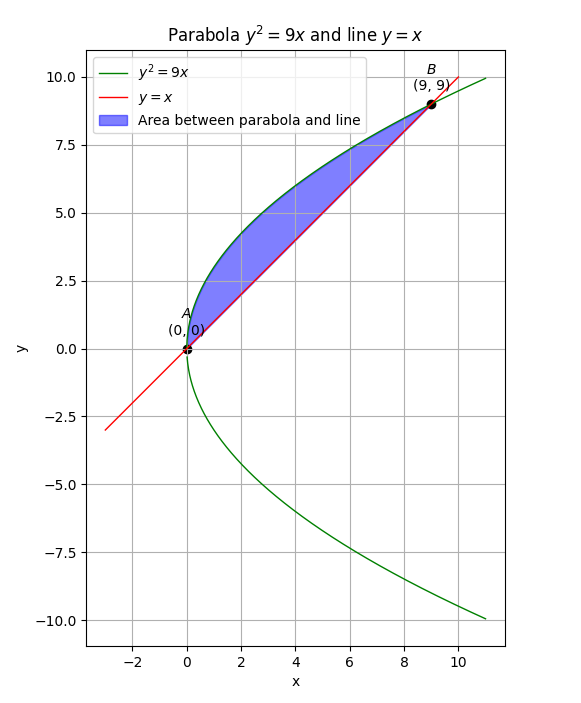
\includegraphics[width=0.5\framewidth]{figs/fig.png}
    \caption{Area between $y^2 = 9x$ and $y=x$}
  \end{figure}
\end{frame}

\section{Codes}
\subsection{C code}
\begin{frame}[fragile,allowframebreaks]
  \frametitle{C code to produce data}
  \begin{mintedbox}{c}[break at=.8\textheight]
#include <stdio.h>
#include <stdlib.h>
#include <math.h>
#include "libs/matfun.h"
#include "libs/geofun.h"

void horizontal_parabola_gen(FILE *fptr, double a, double num_points, double ** vertex) {
  double h = vertex[0][0];
  double k = vertex[1][0];

    for (int i = 0; i <= num_points; i++) {
        double x = (11.0 * i) / num_points; // Scale x from 0 to 11
        double y_pos = k + sqrt(4 * a * (x-h)); // Positive y value
        double y_neg = k - sqrt(4 * a * (x-h)); // Negative y value

        // Output the points for the upper and lower curves
        fprintf(fptr, "%lf,%lf\n", x, y_pos); // Upper
        fprintf(fptr, "%lf,%lf\n", x, y_neg); // Lower
    }
}


int main() {
    double x1, y1;
    x1 = 0; y1 = 0;  // Vertex of the parabola at the origin
    int m = 2, n = 1;
    double **vertex = createMat(m, n);
    vertex[0][0] = x1;
    vertex[1][0] = y1;

    FILE *fptr;
    fptr = fopen("points.txt", "w");
    if (fptr == NULL) {
        printf("Error opening file!\n");
        return 1;
    }

    double a = 9.0/4.0;  // For y^2 = 9x, we have 4a = 9, thus a = 9/4
    horizontal_parabola_gen(fptr, a, 1000, vertex);

    fclose(fptr);
    freeMat(vertex, 2);  // Freeing the dynamically allocated memory
    return 0;
}
  \end{mintedbox}
\end{frame}

\subsection{Python Code}
\begin{frame}[fragile,allowframebreaks]
  \frametitle{Python code to Plot curves}
  \begin{mintedbox}{Python}[break at=.8\textheight]
import sys  # for path to external scripts
sys.path.insert(0, '/Users/hanumac/Desktop/github/matgeo/codes/coordgeo')  # path to GVV Sir's scripts
import numpy as np
import numpy.linalg as LA
import matplotlib.pyplot as plt

# local imports
from line.funcs import *
from triangle.funcs import *
from conics.funcs import circ_gen

# Load the points from the text file generated by the C code
points = np.loadtxt("points.txt", delimiter=',')

# Extract the x and y coordinates
x = points[:, 0]
y = points[:, 1]

# Separate the positive and negative branches of the parabola
x_positive = x[y >= 0]  # X values where y is positive
y_positive = y[y >= 0]  # Positive Y values

x_negative = x[y < 0]   # X values where y is negative
y_negative = y[y < 0]   # Negative Y values

# line parameters
A = np.array(([0, 0]))  # point A
B = np.array(([9, 9]))  # point B
m = np.array(([1, 1])).reshape(-1, 1)  # direction vector of line

# generate line points
line_points = line_dir_pt(m, A.reshape(-1, 1), 10, -3)

# Plot
plt.figure()

# Plot the positive branch of the parabola
plt.plot(x_positive, y_positive, label=r'$y^2 = 9x$', color='green', linewidth=1)

# Plot the negative branch of the parabola
plt.plot(x_negative, y_negative, color='green', linewidth=1)

plt.gca().set_aspect('equal', adjustable='box')

# Plot the line y = x
plt.plot(line_points[0, :], line_points[1, :], label="$ y = x $", color="red", linewidth=1)

# Fill the area between the parabola and the line from x=0 to x=9
x_fill = np.linspace(0, 9, 500)  # X values between 0 and 9
y_parabola = np.sqrt(9 * x_fill)  # Y values for the positive branch of the parabola
y_line = x_fill  # Y values for the line y = x

plt.fill_between(x_fill, y_line, y_parabola, color='blue', alpha=0.5, label='Area between parabola and line')

# Creating coordinates for labeling
tri_coords = np.array([[A[0], B[0]], [A[1], B[1]]])  #array for points
plt.scatter(tri_coords[0, :], tri_coords[1, :], color='black') #Plot points
vert_labels = ['$A$', '$B$']

# Annotate the points using the provided syntax
for i, txt in enumerate(vert_labels):
    plt.annotate(f'{txt}\n({tri_coords[0,i]:.0f}, {tri_coords[1,i]:.0f})',
                 (tri_coords[0,i], tri_coords[1,i]),  # point to label
                 textcoords="offset points",  # position of text
                 xytext=(0, 10),  # distance from text to points (x,y)
                 ha='center')  # horizontal alignment

# Label the axes
plt.xlabel("x")
plt.ylabel("y")
plt.title("Parabola $y^2 = 9x$ and line $y=x$")
plt.grid(True)
plt.legend()
plt.show()
  \end{mintedbox}
\end{frame}


% \begin{comment}
% The code in 
% {\footnotesize
% \begin{lstlisting}
% https://github.com/gadepall/school/blob/master/training/chemistry/codes/chembal.py
% \end{lstlisting}
% }
% \end{comment}

\end{document}
